\documentclass{article}
\usepackage[widepage]{repsty}
\usepackage{subcaption}

\newcommand{\st}{\nu_s}
\newcommand{\nbar}{\bar n}

\begin{document}

\title{Study of spin-orbit motion in the Frozen and Quasi-Frozen rings}
\maketitle

\section{Spin decoherence in a perfectly aligned storage ring}

We study decoherence for two major reasons:
\begin{enumerate}
\item it reduces the measurement time frame;
\item vertical plane decoherence is a source of systematic error.~\cite[p. 8]{Senichev:StorageRingMethod}
\end{enumerate}

In what follows, we consider the decoherence caused by the beam particles' spin tune spread.

The spin dynamics in a storage ring is governed by the FT-BMT equation.~\cite[p. 4]{JEDI:SpinTuneMapping} In the standard spinor formalism, spin evolution is described by a rotation matrix, whose eigenvector is the spin precession axis, $\nbar$, and eigenvalue the spin tune, $\st$. For particles traveling along the design orbit of a perfectly aligned, flat storage ring, the equilibrium direction of $\nbar$ is vertical,~\cite[p. 1362]{DESY:SpinTune} and the spin tune expressions in the electric and magnetic fields are:~\cite[p. 8]{Senichev:StorageRingMethod}
\begin{equation}
  \begin{cases}
    \st^E &= \bkt{\frac1{\gamma^2-1}-G}\gamma\beta^2, \\
    \st^B &= \gamma G,
  \end{cases}
\end{equation}
where $G = \frac{g-2}{2}$ is the magnetic moment anomaly, $\gamma = (1-\beta^2)^{-\sfrac12}$ is the particle's Lorentz factor. Consequently, the spin tune spread is due to the beam particles' equilibrium energy spread. The latter is caused by the finite beam size in phase space.

A non-reference particle is involved in two types of oscillations:
\begin{inparaenum}[a)]
\item betatron, and
\item synchrotron,
\end{inparaenum}
both of which cause orbit-lengthening. The phase stability principle requires that orbit lengthening is accompanied by a corresponding equilibrium level energy shift:~\cite{Senichev:Decoh}
\begin{equation}
  \Delta\delta_{eq} = \frac{\gamma_s^2}{\gamma_s^2\alpha_0 - 1}\bkt*{\frac{\Delta\gamma_m^2}{2}\bkt{\alpha_1 - \frac{\alpha_0}{\gamma_s^2} + \frac{1}{\gamma_s^4}} + \bkt{\frac{\Delta L}{L}}_\beta},
\end{equation}
where $\delta = \frac{\Delta p}{p_s}$ is the particle's momentum deviation, $\Delta\gamma_m$ is its synchrotron oscillation amplitude, $\alpha = \alpha_0 + \alpha_1\delta$ is the momentum compaction factor, $\alpha_0 = \avg{\frac{D_0}{\rho}}$, $\alpha_1 = \avg{\frac{D_1}{\rho}} + \frac12 \avg{D_0^{\prime2}}$, $D_i,~D_i^\prime,~i\in\{0,1\}$ the zero and first order linear and angular dispersion functions respectively, $\rho$ the closed orbit radius, $\bkt{\frac{\Delta L}{L}}_\beta = \frac{\pi}{2L}\bkt*{\varepsilon_x Q_x + \varepsilon_y Q_y}$ the betatron-motion orbit lengthening, $\varepsilon_{x,y}$ the horizontal and vertical emittances, and $Q_{x,y}$ are the betatron tunes.

\section{Decoherence suppression via sextupole fields}
Sextupole fields influence orbit lengthening via two paths:~\cite{Senichev:Decoh}
\begin{enumerate}
\item by modifying the momentum compaction factor: $\Delta\alpha_1 = -\frac{S\cdot D_0^3}{L}$;
\item by directly changing the orbit length: $\frac{\Delta L}{L} = \mp \frac{S\cdot D_0\cdot \beta_{x,y}\varepsilon_{x,y}}{L}$,
\end{enumerate}
where $S$ is the sextupole strength.

For this reason, the orbit-lengthening decoherence can be suppressed by placing three sextupole families (hereinafter called D-, X-, and Y-sextupoles respectively) into the maxima of $D_0,~\beta_x,~\beta_y$ functions.

\section{Simulation}
In order to analyze the effectiveness of sextupole decoherence suppression, a simulation was carried out using the COSY INFINITY code. The perfectly aligned Frozen Spin lattice setup was taken for that purpose, in which we consecutively varied the strengths of the X-, Y-, and D-sextupoles (the strengths of the unvaried families were set to zero), and computed the spin tunes of partices with initial offsets in, respectively, the $x$, $y$, and $\delta \equiv \frac{\Delta K}{K_0}$ coordinates.~\cite{COSYInf:BPManual} This manual search was performed at the energy of 300 MeV, 30 MeV above the ``magic'' energy for the given setup, which is 270 MeV. This was done in order to avoid running into a resonance in the computation of spin tune. After the manual search, further automatic optimization was performed (at the same energy), in order to improve the accuracy.

Since the spin tune has a parabolic dependence on the particle offsets in the $(x,y,\delta)$ coordinates, the figure of merit for the optimization (as well as the manual search) was taken to be the second-order spin tune Taylor expansion coefficient before the corresponding coordinate.

As can be observed from Figure~\ref{fig:OptSext}, use of sextupole fields can remove decoherence in a wide cross-sectional area of the beam pipe.

Of note is the fact that we were not able to suppress decoherence all three types of decohreence simultanteously. Especially problematic is the inclusion of the non-zero GSD gradient. In that case, only the D-type decoherence is suppressed, but both X-, and Y-types become even worse.

\begin{figure}
  \centering
  \begin{subfigure}[b]{\textwidth}\centering
    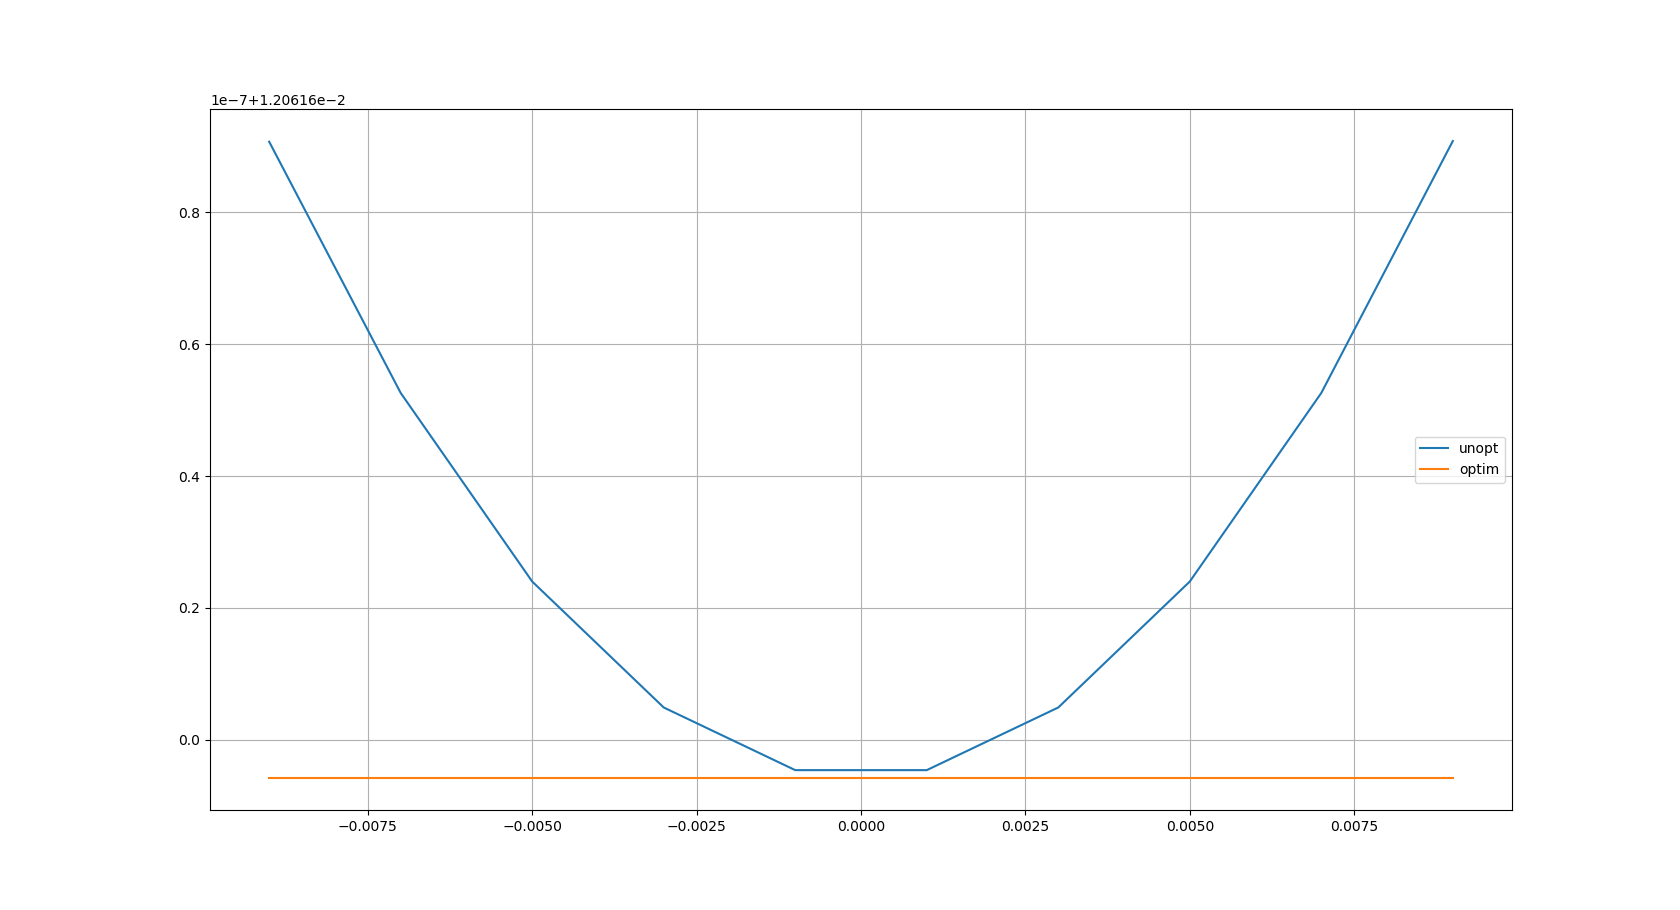
\includegraphics[width=\textwidth]{img/SPINTUNE_X_GSX_optim}
    \caption{GSX optimized for the X bunch}
  \end{subfigure}
  \begin{subfigure}[b]{\textwidth}\centering
    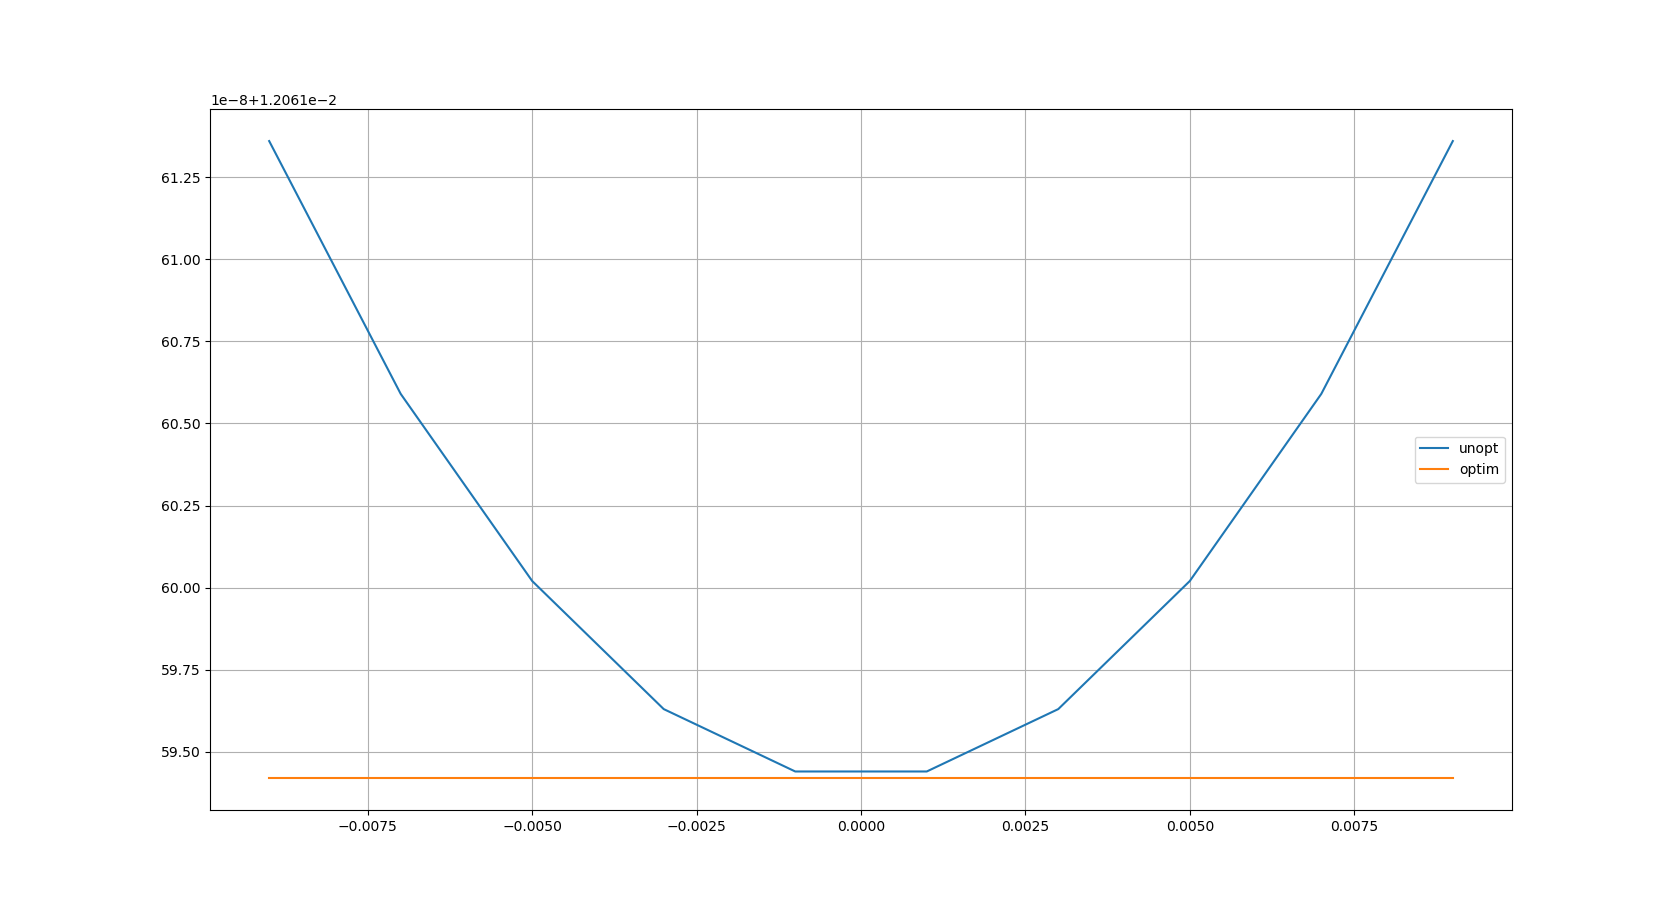
\includegraphics[width=\textwidth]{img/SPINTUNE_Y_GSY_optim}
    \caption{GSY optimized for the Y bunch}
  \end{subfigure}
\end{figure}
\begin{figure}\ContinuedFloat
  \begin{subfigure}[b]{\textwidth}\centering
    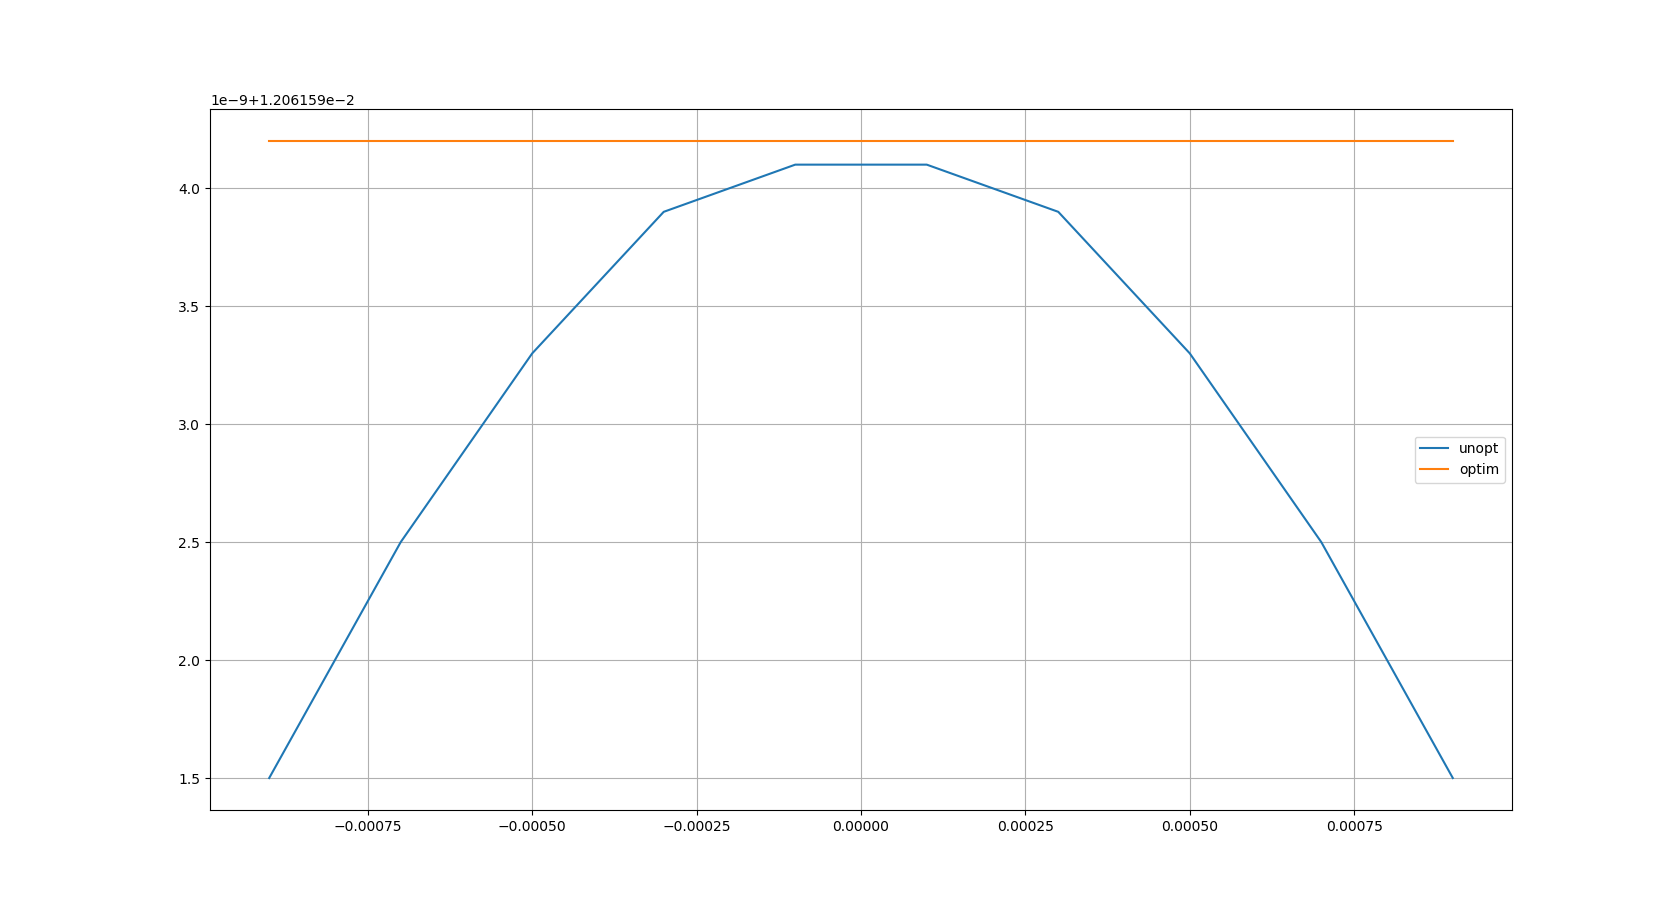
\includegraphics[width=\textwidth]{img/SPINTUNE_D_GSD_optim}
    \caption{GSD optimized for the D bunch}
  \end{subfigure}
  \caption{Spin tunes of offset particles vs the offsets, at 300 MeV, with/out the corresponding sextupole.\label{fig:OptSext}}
\end{figure}

\begin{thebibliography}{99}
\bibitem{JEDI:SpinTuneMapping}
  Saleev A, Nikolaev NN, Rathmann F, Augustyniak W, Bagdasarian Z, Bai M, et al. Spin tune mapping as a novel tool to probe the spin dynamics in storage rings. Physical Review Accelerators and Beams [Internet]. 2017 Jul 7 [cited 2018 Oct 8];20(7). Available from: \url{http://arxiv.org/abs/1703.01295}
  
\bibitem{DESY:SpinTune}
  Barber D P, Vogt M, Hoffst\"atter G H. The Amplitude Dependent Spin Tune and the Invariant Spin Field in High Energy Proton Accelerators. \url{http://accelconf.web.cern.ch/AccelConf/e98/PAPERS/THP35G.PDF}

\bibitem{Senichev:StorageRingMethod}
  Yurij Senichev. Search for the Charged Particle Electric Dipole Moments in Storage Rings. In: 25th Russian Particle Accelerator Conference (RuPAC’16), St Petersburg, Russia, November 21-25, 2016 [Internet]. JACOW, Geneva, Switzerland; 2017 [cited 2017 Apr 5]. p. 6–10. Available from: \url{http://accelconf.web.cern.ch/AccelConf/rupac2016/papers/mozmh03.pdf}

\bibitem{Senichev:Decoh}
  Senichev Y, Zyuzin D. SPIN TUNE DECOHERENCE EFFECTS IN ELECTRO- AND  MAGNETOSTATIC STRUCTURES. In: Beam Dynamics and Electromagnetic Fields [Internet]. Changhai, China: JACoW; 2013 [cited 2017 Jul 31]. p. 2579--2581. Available from: \url{https://accelconf.web.cern.ch/accelconf/IPAC2013/papers/wepea036.pdf}

\bibitem{COSYInf:BPManual}
  Martin Berz, Kyoko Makino. COSY INFINITY 10.0 Beam Physics Manual [Internet]. Michigan State University; 2015 [cited 2017 Mar 20]. Available from: \url{http://cosy.pa.msu.edu/manual/COSYBeamMan100.pdf}

\end{thebibliography}

\end{document}

